\batchmode
\documentclass[twoside]{book}

% Packages required by doxygen
\usepackage{fixltx2e}
\usepackage{calc}
\usepackage{doxygen}
\usepackage[export]{adjustbox} % also loads graphicx
\usepackage{graphicx}
\usepackage[utf8]{inputenc}
\usepackage{makeidx}
\usepackage{multicol}
\usepackage{multirow}
\PassOptionsToPackage{warn}{textcomp}
\usepackage{textcomp}
\usepackage[nointegrals]{wasysym}
\usepackage[table]{xcolor}

% Font selection
\usepackage[T1]{fontenc}
\usepackage[scaled=.90]{helvet}
\usepackage{courier}
\usepackage{amssymb}
\usepackage{sectsty}
\renewcommand{\familydefault}{\sfdefault}
\allsectionsfont{%
  \fontseries{bc}\selectfont%
  \color{darkgray}%
}
\renewcommand{\DoxyLabelFont}{%
  \fontseries{bc}\selectfont%
  \color{darkgray}%
}
\newcommand{\+}{\discretionary{\mbox{\scriptsize$\hookleftarrow$}}{}{}}

% Page & text layout
\usepackage{geometry}
\geometry{%
  a4paper,%
  top=2.5cm,%
  bottom=2.5cm,%
  left=2.5cm,%
  right=2.5cm%
}
\tolerance=750
\hfuzz=15pt
\hbadness=750
\setlength{\emergencystretch}{15pt}
\setlength{\parindent}{0cm}
\setlength{\parskip}{3ex plus 2ex minus 2ex}
\makeatletter
\renewcommand{\paragraph}{%
  \@startsection{paragraph}{4}{0ex}{-1.0ex}{1.0ex}{%
    \normalfont\normalsize\bfseries\SS@parafont%
  }%
}
\renewcommand{\subparagraph}{%
  \@startsection{subparagraph}{5}{0ex}{-1.0ex}{1.0ex}{%
    \normalfont\normalsize\bfseries\SS@subparafont%
  }%
}
\makeatother

% Headers & footers
\usepackage{fancyhdr}
\pagestyle{fancyplain}
\fancyhead[LE]{\fancyplain{}{\bfseries\thepage}}
\fancyhead[CE]{\fancyplain{}{}}
\fancyhead[RE]{\fancyplain{}{\bfseries\leftmark}}
\fancyhead[LO]{\fancyplain{}{\bfseries\rightmark}}
\fancyhead[CO]{\fancyplain{}{}}
\fancyhead[RO]{\fancyplain{}{\bfseries\thepage}}
\fancyfoot[LE]{\fancyplain{}{}}
\fancyfoot[CE]{\fancyplain{}{}}
\fancyfoot[RE]{\fancyplain{}{\bfseries\scriptsize Generated by Doxygen }}
\fancyfoot[LO]{\fancyplain{}{\bfseries\scriptsize Generated by Doxygen }}
\fancyfoot[CO]{\fancyplain{}{}}
\fancyfoot[RO]{\fancyplain{}{}}
\renewcommand{\footrulewidth}{0.4pt}
\renewcommand{\chaptermark}[1]{%
  \markboth{#1}{}%
}
\renewcommand{\sectionmark}[1]{%
  \markright{\thesection\ #1}%
}

% Indices & bibliography
\usepackage{natbib}
\usepackage[titles]{tocloft}
\setcounter{tocdepth}{3}
\setcounter{secnumdepth}{5}
\makeindex

% Hyperlinks (required, but should be loaded last)
\usepackage{ifpdf}
\ifpdf
  \usepackage[pdftex,pagebackref=true]{hyperref}
\else
  \usepackage[ps2pdf,pagebackref=true]{hyperref}
\fi
\hypersetup{%
  colorlinks=true,%
  linkcolor=blue,%
  citecolor=blue,%
  unicode%
}

% Custom commands
\newcommand{\clearemptydoublepage}{%
  \newpage{\pagestyle{empty}\cleardoublepage}%
}

\usepackage{caption}
\captionsetup{labelsep=space,justification=centering,font={bf},singlelinecheck=off,skip=4pt,position=top}

%===== C O N T E N T S =====

\begin{document}

% Titlepage & ToC
\hypersetup{pageanchor=false,
             bookmarksnumbered=true,
             pdfencoding=unicode
            }
\pagenumbering{alph}
\pagenumbering{arabic}
\hypersetup{pageanchor=true}

%--- Begin generated contents ---
\chapter{The Bretherton problem\+: An air finger propagates into a 2D channel}
\label{index}\hypertarget{index}{}\hypertarget{index_q}{}\section{A few quick questions...}\label{index_q}
Since {\ttfamily oomph-\/lib} is developed as open-\/source software, any evidence that the code is being downloaded and used is very helpful for us as it helps to justify our continued work on this project.

We would therefore be extremely grateful if you could provide the information requested in the form below. Pressing the \char`\"{}submit\char`\"{} button will get you to the actual download page.

{\bfseries Note\+:} 
\begin{DoxyItemize}
\item All information will be treated as confidential. 
\item If you provide your email address and check the appropriate box we will add you to our mailing list to inform you of upgrades and bug fixes to the code. Rest assured that the mailing list is {\bfseries very low volume} -- we have better things to do than to bombard you with email. 
\item If you still feel reluctant to provide any of the information requested, feel free to enter some dummy input. The form will check that {\bfseries some} information has been entered but entering your name as \char`\"{}\+Joe Cool\char`\"{} is perfectly acceptable -- this is to discourage people from not providing the information simply because they are too lazy to type... 
\end{DoxyItemize}



 







 

 \hypertarget{index_pdf}{}\section{P\+D\+F file}\label{index_pdf}
A \href{../latex/refman.pdf}{\tt pdf version} of this document is available. \end{document}

\chapter{Namespace Index}
\section{Namespace List}
Here is a list of all namespaces with brief descriptions\+:\begin{DoxyCompactList}
\item\contentsline{section}{\hyperlink{namespaceGlobal__Physical__Variables}{Global\+\_\+\+Physical\+\_\+\+Variables} \\*Global variables that represent physical properties }{\pageref{namespaceGlobal__Physical__Variables}}{}
\item\contentsline{section}{\hyperlink{namespaceoomph}{oomph} }{\pageref{namespaceoomph}}{}
\item\contentsline{section}{\hyperlink{namespacePhysical__Variables}{Physical\+\_\+\+Variables} \\*Namespace for the solution of 2D linear shell equation }{\pageref{namespacePhysical__Variables}}{}
\end{DoxyCompactList}

\chapter{Hierarchical Index}
\section{Class Hierarchy}
This inheritance list is sorted roughly, but not completely, alphabetically\+:\begin{DoxyCompactList}
\item Problem\begin{DoxyCompactList}
\item \contentsline{section}{Unstructured\+Solid\+Problem$<$ E\+L\+E\+M\+E\+NT $>$}{\pageref{classUnstructuredSolidProblem}}{}
\end{DoxyCompactList}
\end{DoxyCompactList}

\chapter{Class Index}
\section{Class List}
Here are the classes, structs, unions and interfaces with brief descriptions\+:\begin{DoxyCompactList}
\item\contentsline{section}{\hyperlink{classPMLProblem}{P\+M\+L\+Problem$<$ E\+L\+E\+M\+E\+N\+T $>$} }{\pageref{classPMLProblem}}{}
\item\contentsline{section}{\hyperlink{classGlobalParameters_1_1TestPMLMapping}{Global\+Parameters\+::\+Test\+P\+M\+L\+Mapping} }{\pageref{classGlobalParameters_1_1TestPMLMapping}}{}
\end{DoxyCompactList}

\chapter{File Index}
\section{File List}
Here is a list of all files with brief descriptions\+:\begin{DoxyCompactList}
\item\contentsline{section}{\hyperlink{jeffery__orbit_8cc}{jeffery\+\_\+orbit.\+cc} }{\pageref{jeffery__orbit_8cc}}{}
\item\contentsline{section}{\hyperlink{jeffery__orbit_8txt__doxygenified_8h}{jeffery\+\_\+orbit.\+txt\+\_\+doxygenified.\+h} }{\pageref{jeffery__orbit_8txt__doxygenified_8h}}{}
\item\contentsline{section}{\hyperlink{my__taylor__hood__elements_8h}{my\+\_\+taylor\+\_\+hood\+\_\+elements.\+h} }{\pageref{my__taylor__hood__elements_8h}}{}
\end{DoxyCompactList}

\chapter{Namespace Documentation}
\hypertarget{namespaceGlobal__Physical__Variables}{}\section{Global\+\_\+\+Physical\+\_\+\+Variables Namespace Reference}
\label{namespaceGlobal__Physical__Variables}\index{Global\+\_\+\+Physical\+\_\+\+Variables@{Global\+\_\+\+Physical\+\_\+\+Variables}}


Namespace for physical parameters.  


\subsection*{Functions}
\begin{DoxyCompactItemize}
\item 
Vector$<$ double $>$ \hyperlink{namespaceGlobal__Physical__Variables_afae321364975eb56688ad13abc8ed6b7}{Gravity} (2)
\begin{DoxyCompactList}\small\item\em Gravity vector. \end{DoxyCompactList}\item 
void \hyperlink{namespaceGlobal__Physical__Variables_a87da705b8a46bed337cf5dbdd788b87b}{body\+\_\+force} (const double \&time, const Vector$<$ double $>$ \&x, Vector$<$ double $>$ \&result)
\begin{DoxyCompactList}\small\item\em Functional body force. \end{DoxyCompactList}\item 
void \hyperlink{namespaceGlobal__Physical__Variables_a9780d615ae07c4e00a436ab2973b54e6}{zero\+\_\+body\+\_\+force} (const double \&time, const Vector$<$ double $>$ \&x, Vector$<$ double $>$ \&result)
\begin{DoxyCompactList}\small\item\em Zero functional body force. \end{DoxyCompactList}\end{DoxyCompactItemize}
\subsection*{Variables}
\begin{DoxyCompactItemize}
\item 
double \hyperlink{namespaceGlobal__Physical__Variables_ab814e627d2eb5bc50318879d19ab16b9}{Re} =100
\begin{DoxyCompactList}\small\item\em Reynolds number. \end{DoxyCompactList}\item 
double \hyperlink{namespaceGlobal__Physical__Variables_ab1a845a672b4d74b304639a976dc65c6}{Re\+\_\+inv\+Fr} =100
\begin{DoxyCompactList}\small\item\em Reynolds/\+Froude number. \end{DoxyCompactList}\end{DoxyCompactItemize}


\subsection{Detailed Description}
Namespace for physical parameters. 

\subsection{Function Documentation}
\mbox{\Hypertarget{namespaceGlobal__Physical__Variables_a87da705b8a46bed337cf5dbdd788b87b}\label{namespaceGlobal__Physical__Variables_a87da705b8a46bed337cf5dbdd788b87b}} 
\index{Global\+\_\+\+Physical\+\_\+\+Variables@{Global\+\_\+\+Physical\+\_\+\+Variables}!body\+\_\+force@{body\+\_\+force}}
\index{body\+\_\+force@{body\+\_\+force}!Global\+\_\+\+Physical\+\_\+\+Variables@{Global\+\_\+\+Physical\+\_\+\+Variables}}
\subsubsection{\texorpdfstring{body\+\_\+force()}{body\_force()}}
{\footnotesize\ttfamily void Global\+\_\+\+Physical\+\_\+\+Variables\+::body\+\_\+force (\begin{DoxyParamCaption}\item[{const double \&}]{time,  }\item[{const Vector$<$ double $>$ \&}]{x,  }\item[{Vector$<$ double $>$ \&}]{result }\end{DoxyParamCaption})}



Functional body force. 



Definition at line 62 of file circular\+\_\+driven\+\_\+cavity.\+cc.



References Re\+\_\+inv\+Fr.



Referenced by main().

\mbox{\Hypertarget{namespaceGlobal__Physical__Variables_afae321364975eb56688ad13abc8ed6b7}\label{namespaceGlobal__Physical__Variables_afae321364975eb56688ad13abc8ed6b7}} 
\index{Global\+\_\+\+Physical\+\_\+\+Variables@{Global\+\_\+\+Physical\+\_\+\+Variables}!Gravity@{Gravity}}
\index{Gravity@{Gravity}!Global\+\_\+\+Physical\+\_\+\+Variables@{Global\+\_\+\+Physical\+\_\+\+Variables}}
\subsubsection{\texorpdfstring{Gravity()}{Gravity()}}
{\footnotesize\ttfamily Vector$<$double$>$ Global\+\_\+\+Physical\+\_\+\+Variables\+::\+Gravity (\begin{DoxyParamCaption}\item[{2}]{ }\end{DoxyParamCaption})}



Gravity vector. 



Referenced by main(), and Quarter\+Circle\+Driven\+Cavity\+Problem$<$ E\+L\+E\+M\+E\+N\+T $>$\+::\+Quarter\+Circle\+Driven\+Cavity\+Problem().

\mbox{\Hypertarget{namespaceGlobal__Physical__Variables_a9780d615ae07c4e00a436ab2973b54e6}\label{namespaceGlobal__Physical__Variables_a9780d615ae07c4e00a436ab2973b54e6}} 
\index{Global\+\_\+\+Physical\+\_\+\+Variables@{Global\+\_\+\+Physical\+\_\+\+Variables}!zero\+\_\+body\+\_\+force@{zero\+\_\+body\+\_\+force}}
\index{zero\+\_\+body\+\_\+force@{zero\+\_\+body\+\_\+force}!Global\+\_\+\+Physical\+\_\+\+Variables@{Global\+\_\+\+Physical\+\_\+\+Variables}}
\subsubsection{\texorpdfstring{zero\+\_\+body\+\_\+force()}{zero\_body\_force()}}
{\footnotesize\ttfamily void Global\+\_\+\+Physical\+\_\+\+Variables\+::zero\+\_\+body\+\_\+force (\begin{DoxyParamCaption}\item[{const double \&}]{time,  }\item[{const Vector$<$ double $>$ \&}]{x,  }\item[{Vector$<$ double $>$ \&}]{result }\end{DoxyParamCaption})}



Zero functional body force. 



Definition at line 70 of file circular\+\_\+driven\+\_\+cavity.\+cc.



Referenced by main().



\subsection{Variable Documentation}
\mbox{\Hypertarget{namespaceGlobal__Physical__Variables_ab814e627d2eb5bc50318879d19ab16b9}\label{namespaceGlobal__Physical__Variables_ab814e627d2eb5bc50318879d19ab16b9}} 
\index{Global\+\_\+\+Physical\+\_\+\+Variables@{Global\+\_\+\+Physical\+\_\+\+Variables}!Re@{Re}}
\index{Re@{Re}!Global\+\_\+\+Physical\+\_\+\+Variables@{Global\+\_\+\+Physical\+\_\+\+Variables}}
\subsubsection{\texorpdfstring{Re}{Re}}
{\footnotesize\ttfamily double Global\+\_\+\+Physical\+\_\+\+Variables\+::\+Re =100}



Reynolds number. 



Definition at line 53 of file circular\+\_\+driven\+\_\+cavity.\+cc.



Referenced by Quarter\+Circle\+Driven\+Cavity\+Problem$<$ E\+L\+E\+M\+E\+N\+T $>$\+::\+Quarter\+Circle\+Driven\+Cavity\+Problem().

\mbox{\Hypertarget{namespaceGlobal__Physical__Variables_ab1a845a672b4d74b304639a976dc65c6}\label{namespaceGlobal__Physical__Variables_ab1a845a672b4d74b304639a976dc65c6}} 
\index{Global\+\_\+\+Physical\+\_\+\+Variables@{Global\+\_\+\+Physical\+\_\+\+Variables}!Re\+\_\+inv\+Fr@{Re\+\_\+inv\+Fr}}
\index{Re\+\_\+inv\+Fr@{Re\+\_\+inv\+Fr}!Global\+\_\+\+Physical\+\_\+\+Variables@{Global\+\_\+\+Physical\+\_\+\+Variables}}
\subsubsection{\texorpdfstring{Re\+\_\+inv\+Fr}{Re\_invFr}}
{\footnotesize\ttfamily double Global\+\_\+\+Physical\+\_\+\+Variables\+::\+Re\+\_\+inv\+Fr =100}



Reynolds/\+Froude number. 



Definition at line 56 of file circular\+\_\+driven\+\_\+cavity.\+cc.



Referenced by body\+\_\+force(), and Quarter\+Circle\+Driven\+Cavity\+Problem$<$ E\+L\+E\+M\+E\+N\+T $>$\+::\+Quarter\+Circle\+Driven\+Cavity\+Problem().


\hypertarget{namespaceoomph}{}\section{oomph Namespace Reference}
\label{namespaceoomph}\index{oomph@{oomph}}
\subsection*{Classes}
\begin{DoxyCompactItemize}
\item 
class \hyperlink{classoomph_1_1BellShellElement}{Bell\+Shell\+Element}
\begin{DoxyCompactList}\small\item\em \hyperlink{classoomph_1_1BellShellElement}{Bell\+Shell\+Element} elements are with subparametric interpolation for the function. \end{DoxyCompactList}\item 
class \hyperlink{classoomph_1_1FaceGeometry_3_01BellShellElement_3_01DIM_00_01NNODE__1D_01_4_01_4}{Face\+Geometry$<$ Bell\+Shell\+Element$<$ D\+I\+M, N\+N\+O\+D\+E\+\_\+1\+D $>$ $>$}
\item 
class \hyperlink{classoomph_1_1MyShellEquations}{My\+Shell\+Equations}
\item 
class \hyperlink{classoomph_1_1Plate}{Plate}
\begin{DoxyCompactList}\small\item\em Elliptical tube with half axes a and b. \end{DoxyCompactList}\end{DoxyCompactItemize}

\chapter{Class Documentation}
\hypertarget{classBrethertonElement}{}\section{Bretherton\+Element$<$ E\+L\+E\+M\+E\+NT $>$ Class Template Reference}
\label{classBrethertonElement}\index{Bretherton\+Element$<$ E\+L\+E\+M\+E\+N\+T $>$@{Bretherton\+Element$<$ E\+L\+E\+M\+E\+N\+T $>$}}
Inheritance diagram for Bretherton\+Element$<$ E\+L\+E\+M\+E\+NT $>$\+:\begin{figure}[H]
\begin{center}
\leavevmode
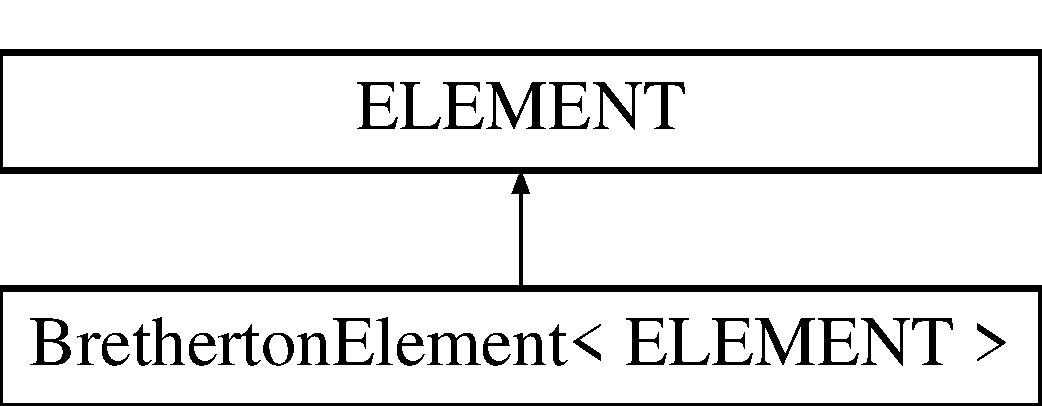
\includegraphics[height=2.000000cm]{classBrethertonElement}
\end{center}
\end{figure}
\subsection*{Public Types}
\begin{DoxyCompactItemize}
\item 
typedef void($\ast$ \hyperlink{classBrethertonElement_a313d868ce6fbd8df07b0360db25133ce}{Inflow\+Fct\+Pt}) (const Vector$<$ double $>$ \&x, Vector$<$ double $>$ \&veloc)
\begin{DoxyCompactList}\small\item\em Typedef for pointer (global) function that specifies the the inflow. \end{DoxyCompactList}\end{DoxyCompactItemize}
\subsection*{Public Member Functions}
\begin{DoxyCompactItemize}
\item 
\hyperlink{classBrethertonElement_acbc668eed3ea683a67b6b822d6e59974}{Bretherton\+Element} ()
\begin{DoxyCompactList}\small\item\em Constructor\+: Call the constructor of the underlying element. \end{DoxyCompactList}\item 
void \hyperlink{classBrethertonElement_aa526749ab70cd15ee05c1b58b5f135a6}{activate\+\_\+inflow\+\_\+dependency\+\_\+on\+\_\+external\+\_\+data} (const Vector$<$ Data $\ast$$>$ \&inflow\+\_\+ext\+\_\+data, const unsigned \&inflow\+\_\+boundary, \hyperlink{classBrethertonElement_a313d868ce6fbd8df07b0360db25133ce}{Inflow\+Fct\+Pt} inflow\+\_\+fct\+\_\+pt)
\begin{DoxyCompactList}\small\item\em Activate the dependency of the \char`\"{}inflow\char`\"{} on the external data. Pass the vector of pointers to the external Data that affects the inflow, the id of the boundary on which the inflow condition is to be applied and the function pointer to to the global function that defines the inflow. \end{DoxyCompactList}\item 
void \hyperlink{classBrethertonElement_a40f35d9e03eae08954b6b32badadcf61}{assign\+\_\+local\+\_\+eqn\+\_\+numbers} (const bool \&store\+\_\+local\+\_\+dof\+\_\+pt)
\item 
void \hyperlink{classBrethertonElement_ab0bc00d862b2c888703ed38c74f18b77}{get\+\_\+jacobian} (Vector$<$ double $>$ \&residuals, Dense\+Matrix$<$ double $>$ \&jacobian)
\end{DoxyCompactItemize}
\subsection*{Private Member Functions}
\begin{DoxyCompactItemize}
\item 
void \hyperlink{classBrethertonElement_a7e655df2ed6104862cc70c2408daf93c}{reassign\+\_\+inflow} ()
\begin{DoxyCompactList}\small\item\em For all nodes that are located on specified boundary re-\/assign the inflow velocity, using the function pointed to by the function pointer. \end{DoxyCompactList}\end{DoxyCompactItemize}
\subsection*{Private Attributes}
\begin{DoxyCompactItemize}
\item 
Vector$<$ Data $\ast$ $>$ \hyperlink{classBrethertonElement_a84c7822cf2a97fe45e936429faa16788}{Inflow\+\_\+ext\+\_\+data}
\begin{DoxyCompactList}\small\item\em Storage for the external Data that affects the inflow. \end{DoxyCompactList}\item 
Dense\+Matrix$<$ int $>$ \hyperlink{classBrethertonElement_ad1ddf8c7a6fd590bf7156d13640303d1}{Inflow\+\_\+ext\+\_\+data\+\_\+eqn}
\begin{DoxyCompactList}\small\item\em Storage for the local equation numbers associated the Data values that affect the inflow. \end{DoxyCompactList}\item 
unsigned \hyperlink{classBrethertonElement_a2d3a3d4837d41865d5f62271c98715c5}{Inflow\+\_\+boundary}
\begin{DoxyCompactList}\small\item\em Number of the inflow boundary in the global mesh. \end{DoxyCompactList}\item 
\hyperlink{classBrethertonElement_a313d868ce6fbd8df07b0360db25133ce}{Inflow\+Fct\+Pt} \hyperlink{classBrethertonElement_a6ded0faba9d7fcfe96834c56af461977}{Inflow\+\_\+fct\+\_\+pt}
\begin{DoxyCompactList}\small\item\em Function pointer to the global function that specifies the inflow velocity profile on the global mesh boundary Inflow\+\_\+boundary. \end{DoxyCompactList}\end{DoxyCompactItemize}


\subsection{Detailed Description}
\subsubsection*{template$<$class E\+L\+E\+M\+E\+NT$>$\newline
class Bretherton\+Element$<$ E\+L\+E\+M\+E\+N\+T $>$}

\char`\"{}\+Bretherton element\char`\"{} is a fluid element (of type E\+L\+E\+M\+E\+NT) for which the (inflow) velocity at those nodes that are located on a specified Mesh boundary is prescribed by Dirichlet boundary conditions. The key is that prescribed velocity profile can be a function of some external Data -- this dependency must be taken into account when computing the element\textquotesingle{}s Jacobian matrix.

This element type is useful, for instance, in the Bretherton problem, where the parabolic \char`\"{}inflow\char`\"{} profile is a function of the film thickness (represented by Spine heights) at the \char`\"{}outflow\char`\"{}. 

Definition at line 157 of file bretherton.\+cc.



\subsection{Member Typedef Documentation}
\mbox{\Hypertarget{classBrethertonElement_a313d868ce6fbd8df07b0360db25133ce}\label{classBrethertonElement_a313d868ce6fbd8df07b0360db25133ce}} 
\index{Bretherton\+Element@{Bretherton\+Element}!Inflow\+Fct\+Pt@{Inflow\+Fct\+Pt}}
\index{Inflow\+Fct\+Pt@{Inflow\+Fct\+Pt}!Bretherton\+Element@{Bretherton\+Element}}
\subsubsection{\texorpdfstring{Inflow\+Fct\+Pt}{InflowFctPt}}
{\footnotesize\ttfamily template$<$class E\+L\+E\+M\+E\+NT $>$ \\
typedef void($\ast$ \hyperlink{classBrethertonElement}{Bretherton\+Element}$<$ E\+L\+E\+M\+E\+NT $>$\+::Inflow\+Fct\+Pt) (const Vector$<$ double $>$ \&x, Vector$<$ double $>$ \&veloc)}



Typedef for pointer (global) function that specifies the the inflow. 



Definition at line 164 of file bretherton.\+cc.



\subsection{Constructor \& Destructor Documentation}
\mbox{\Hypertarget{classBrethertonElement_acbc668eed3ea683a67b6b822d6e59974}\label{classBrethertonElement_acbc668eed3ea683a67b6b822d6e59974}} 
\index{Bretherton\+Element@{Bretherton\+Element}!Bretherton\+Element@{Bretherton\+Element}}
\index{Bretherton\+Element@{Bretherton\+Element}!Bretherton\+Element@{Bretherton\+Element}}
\subsubsection{\texorpdfstring{Bretherton\+Element()}{BrethertonElement()}}
{\footnotesize\ttfamily template$<$class E\+L\+E\+M\+E\+NT $>$ \\
\hyperlink{classBrethertonElement}{Bretherton\+Element}$<$ E\+L\+E\+M\+E\+NT $>$\+::\hyperlink{classBrethertonElement}{Bretherton\+Element} (\begin{DoxyParamCaption}{ }\end{DoxyParamCaption})\hspace{0.3cm}{\ttfamily [inline]}}



Constructor\+: Call the constructor of the underlying element. 



Definition at line 167 of file bretherton.\+cc.



\subsection{Member Function Documentation}
\mbox{\Hypertarget{classBrethertonElement_aa526749ab70cd15ee05c1b58b5f135a6}\label{classBrethertonElement_aa526749ab70cd15ee05c1b58b5f135a6}} 
\index{Bretherton\+Element@{Bretherton\+Element}!activate\+\_\+inflow\+\_\+dependency\+\_\+on\+\_\+external\+\_\+data@{activate\+\_\+inflow\+\_\+dependency\+\_\+on\+\_\+external\+\_\+data}}
\index{activate\+\_\+inflow\+\_\+dependency\+\_\+on\+\_\+external\+\_\+data@{activate\+\_\+inflow\+\_\+dependency\+\_\+on\+\_\+external\+\_\+data}!Bretherton\+Element@{Bretherton\+Element}}
\subsubsection{\texorpdfstring{activate\+\_\+inflow\+\_\+dependency\+\_\+on\+\_\+external\+\_\+data()}{activate\_inflow\_dependency\_on\_external\_data()}}
{\footnotesize\ttfamily template$<$class E\+L\+E\+M\+E\+NT $>$ \\
void \hyperlink{classBrethertonElement}{Bretherton\+Element}$<$ E\+L\+E\+M\+E\+NT $>$\+::activate\+\_\+inflow\+\_\+dependency\+\_\+on\+\_\+external\+\_\+data (\begin{DoxyParamCaption}\item[{const Vector$<$ Data $\ast$$>$ \&}]{inflow\+\_\+ext\+\_\+data,  }\item[{const unsigned \&}]{inflow\+\_\+boundary,  }\item[{\hyperlink{classBrethertonElement_a313d868ce6fbd8df07b0360db25133ce}{Inflow\+Fct\+Pt}}]{inflow\+\_\+fct\+\_\+pt }\end{DoxyParamCaption})\hspace{0.3cm}{\ttfamily [inline]}}



Activate the dependency of the \char`\"{}inflow\char`\"{} on the external data. Pass the vector of pointers to the external Data that affects the inflow, the id of the boundary on which the inflow condition is to be applied and the function pointer to to the global function that defines the inflow. 



Definition at line 175 of file bretherton.\+cc.

\mbox{\Hypertarget{classBrethertonElement_a40f35d9e03eae08954b6b32badadcf61}\label{classBrethertonElement_a40f35d9e03eae08954b6b32badadcf61}} 
\index{Bretherton\+Element@{Bretherton\+Element}!assign\+\_\+local\+\_\+eqn\+\_\+numbers@{assign\+\_\+local\+\_\+eqn\+\_\+numbers}}
\index{assign\+\_\+local\+\_\+eqn\+\_\+numbers@{assign\+\_\+local\+\_\+eqn\+\_\+numbers}!Bretherton\+Element@{Bretherton\+Element}}
\subsubsection{\texorpdfstring{assign\+\_\+local\+\_\+eqn\+\_\+numbers()}{assign\_local\_eqn\_numbers()}}
{\footnotesize\ttfamily template$<$class E\+L\+E\+M\+E\+NT $>$ \\
void \hyperlink{classBrethertonElement}{Bretherton\+Element}$<$ E\+L\+E\+M\+E\+NT $>$\+::assign\+\_\+local\+\_\+eqn\+\_\+numbers (\begin{DoxyParamCaption}\item[{const bool \&}]{store\+\_\+local\+\_\+dof\+\_\+pt }\end{DoxyParamCaption})\hspace{0.3cm}{\ttfamily [inline]}}

short Overload assign local equation numbers\+: Add the dependency on the external Data that affects the inflow profile 

Definition at line 196 of file bretherton.\+cc.

\mbox{\Hypertarget{classBrethertonElement_ab0bc00d862b2c888703ed38c74f18b77}\label{classBrethertonElement_ab0bc00d862b2c888703ed38c74f18b77}} 
\index{Bretherton\+Element@{Bretherton\+Element}!get\+\_\+jacobian@{get\+\_\+jacobian}}
\index{get\+\_\+jacobian@{get\+\_\+jacobian}!Bretherton\+Element@{Bretherton\+Element}}
\subsubsection{\texorpdfstring{get\+\_\+jacobian()}{get\_jacobian()}}
{\footnotesize\ttfamily template$<$class E\+L\+E\+M\+E\+NT $>$ \\
void \hyperlink{classBrethertonElement}{Bretherton\+Element}$<$ E\+L\+E\+M\+E\+NT $>$\+::get\+\_\+jacobian (\begin{DoxyParamCaption}\item[{Vector$<$ double $>$ \&}]{residuals,  }\item[{Dense\+Matrix$<$ double $>$ \&}]{jacobian }\end{DoxyParamCaption})\hspace{0.3cm}{\ttfamily [inline]}}

Overloaded Jacobian computation\+: Computes the Jacobian of the underlying element and then adds the FD operations to evaluate the derivatives w.\+r.\+t. the Data values that affect the inflow. 

Definition at line 265 of file bretherton.\+cc.

\mbox{\Hypertarget{classBrethertonElement_a7e655df2ed6104862cc70c2408daf93c}\label{classBrethertonElement_a7e655df2ed6104862cc70c2408daf93c}} 
\index{Bretherton\+Element@{Bretherton\+Element}!reassign\+\_\+inflow@{reassign\+\_\+inflow}}
\index{reassign\+\_\+inflow@{reassign\+\_\+inflow}!Bretherton\+Element@{Bretherton\+Element}}
\subsubsection{\texorpdfstring{reassign\+\_\+inflow()}{reassign\_inflow()}}
{\footnotesize\ttfamily template$<$class E\+L\+E\+M\+E\+NT $>$ \\
void \hyperlink{classBrethertonElement}{Bretherton\+Element}$<$ E\+L\+E\+M\+E\+NT $>$\+::reassign\+\_\+inflow (\begin{DoxyParamCaption}{ }\end{DoxyParamCaption})\hspace{0.3cm}{\ttfamily [inline]}, {\ttfamily [private]}}



For all nodes that are located on specified boundary re-\/assign the inflow velocity, using the function pointed to by the function pointer. 



Definition at line 343 of file bretherton.\+cc.



\subsection{Member Data Documentation}
\mbox{\Hypertarget{classBrethertonElement_a2d3a3d4837d41865d5f62271c98715c5}\label{classBrethertonElement_a2d3a3d4837d41865d5f62271c98715c5}} 
\index{Bretherton\+Element@{Bretherton\+Element}!Inflow\+\_\+boundary@{Inflow\+\_\+boundary}}
\index{Inflow\+\_\+boundary@{Inflow\+\_\+boundary}!Bretherton\+Element@{Bretherton\+Element}}
\subsubsection{\texorpdfstring{Inflow\+\_\+boundary}{Inflow\_boundary}}
{\footnotesize\ttfamily template$<$class E\+L\+E\+M\+E\+NT $>$ \\
unsigned \hyperlink{classBrethertonElement}{Bretherton\+Element}$<$ E\+L\+E\+M\+E\+NT $>$\+::Inflow\+\_\+boundary\hspace{0.3cm}{\ttfamily [private]}}



Number of the inflow boundary in the global mesh. 



Definition at line 394 of file bretherton.\+cc.

\mbox{\Hypertarget{classBrethertonElement_a84c7822cf2a97fe45e936429faa16788}\label{classBrethertonElement_a84c7822cf2a97fe45e936429faa16788}} 
\index{Bretherton\+Element@{Bretherton\+Element}!Inflow\+\_\+ext\+\_\+data@{Inflow\+\_\+ext\+\_\+data}}
\index{Inflow\+\_\+ext\+\_\+data@{Inflow\+\_\+ext\+\_\+data}!Bretherton\+Element@{Bretherton\+Element}}
\subsubsection{\texorpdfstring{Inflow\+\_\+ext\+\_\+data}{Inflow\_ext\_data}}
{\footnotesize\ttfamily template$<$class E\+L\+E\+M\+E\+NT $>$ \\
Vector$<$Data$\ast$$>$ \hyperlink{classBrethertonElement}{Bretherton\+Element}$<$ E\+L\+E\+M\+E\+NT $>$\+::Inflow\+\_\+ext\+\_\+data\hspace{0.3cm}{\ttfamily [private]}}



Storage for the external Data that affects the inflow. 



Definition at line 387 of file bretherton.\+cc.

\mbox{\Hypertarget{classBrethertonElement_ad1ddf8c7a6fd590bf7156d13640303d1}\label{classBrethertonElement_ad1ddf8c7a6fd590bf7156d13640303d1}} 
\index{Bretherton\+Element@{Bretherton\+Element}!Inflow\+\_\+ext\+\_\+data\+\_\+eqn@{Inflow\+\_\+ext\+\_\+data\+\_\+eqn}}
\index{Inflow\+\_\+ext\+\_\+data\+\_\+eqn@{Inflow\+\_\+ext\+\_\+data\+\_\+eqn}!Bretherton\+Element@{Bretherton\+Element}}
\subsubsection{\texorpdfstring{Inflow\+\_\+ext\+\_\+data\+\_\+eqn}{Inflow\_ext\_data\_eqn}}
{\footnotesize\ttfamily template$<$class E\+L\+E\+M\+E\+NT $>$ \\
Dense\+Matrix$<$int$>$ \hyperlink{classBrethertonElement}{Bretherton\+Element}$<$ E\+L\+E\+M\+E\+NT $>$\+::Inflow\+\_\+ext\+\_\+data\+\_\+eqn\hspace{0.3cm}{\ttfamily [private]}}



Storage for the local equation numbers associated the Data values that affect the inflow. 



Definition at line 391 of file bretherton.\+cc.

\mbox{\Hypertarget{classBrethertonElement_a6ded0faba9d7fcfe96834c56af461977}\label{classBrethertonElement_a6ded0faba9d7fcfe96834c56af461977}} 
\index{Bretherton\+Element@{Bretherton\+Element}!Inflow\+\_\+fct\+\_\+pt@{Inflow\+\_\+fct\+\_\+pt}}
\index{Inflow\+\_\+fct\+\_\+pt@{Inflow\+\_\+fct\+\_\+pt}!Bretherton\+Element@{Bretherton\+Element}}
\subsubsection{\texorpdfstring{Inflow\+\_\+fct\+\_\+pt}{Inflow\_fct\_pt}}
{\footnotesize\ttfamily template$<$class E\+L\+E\+M\+E\+NT $>$ \\
\hyperlink{classBrethertonElement_a313d868ce6fbd8df07b0360db25133ce}{Inflow\+Fct\+Pt} \hyperlink{classBrethertonElement}{Bretherton\+Element}$<$ E\+L\+E\+M\+E\+NT $>$\+::Inflow\+\_\+fct\+\_\+pt\hspace{0.3cm}{\ttfamily [private]}}



Function pointer to the global function that specifies the inflow velocity profile on the global mesh boundary Inflow\+\_\+boundary. 



Definition at line 398 of file bretherton.\+cc.



The documentation for this class was generated from the following file\+:\begin{DoxyCompactItemize}
\item 
\hyperlink{bretherton_8cc}{bretherton.\+cc}\end{DoxyCompactItemize}

\hypertarget{classBrethertonProblem}{}\section{Bretherton\+Problem$<$ E\+L\+E\+M\+E\+NT $>$ Class Template Reference}
\label{classBrethertonProblem}\index{Bretherton\+Problem$<$ E\+L\+E\+M\+E\+N\+T $>$@{Bretherton\+Problem$<$ E\+L\+E\+M\+E\+N\+T $>$}}


Bretherton problem.  


Inheritance diagram for Bretherton\+Problem$<$ E\+L\+E\+M\+E\+NT $>$\+:\begin{figure}[H]
\begin{center}
\leavevmode
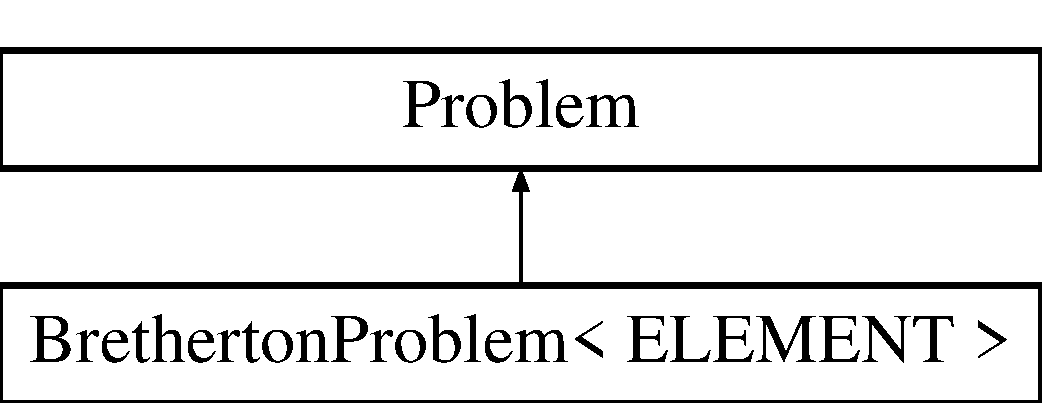
\includegraphics[height=2.000000cm]{classBrethertonProblem}
\end{center}
\end{figure}
\subsection*{Public Member Functions}
\begin{DoxyCompactItemize}
\item 
\hyperlink{classBrethertonProblem_a207cdfe4cf60e83257e759b1ac15e5eb}{Bretherton\+Problem} ()
\begin{DoxyCompactList}\small\item\em Constructor\+: \end{DoxyCompactList}\item 
void \hyperlink{classBrethertonProblem_a6a3e76e4900715d8c2fd15d0e350d724}{actions\+\_\+before\+\_\+newton\+\_\+convergence\+\_\+check} ()
\begin{DoxyCompactList}\small\item\em Spine heights/lengths are unknowns in the problem so their values get corrected during each Newton step. However, changing their value does not automatically change the nodal positions, so we need to update all of them. \end{DoxyCompactList}\item 
void \hyperlink{classBrethertonProblem_a7112e0efe4c0cd0269cf47f02df4fe22}{actions\+\_\+before\+\_\+newton\+\_\+solve} ()
\begin{DoxyCompactList}\small\item\em Update before solve\+: empty. \end{DoxyCompactList}\item 
void \hyperlink{classBrethertonProblem_a2e84e3ce784b0f0de5eeefe1175d48ff}{actions\+\_\+after\+\_\+newton\+\_\+solve} ()
\begin{DoxyCompactList}\small\item\em Update after solve can remain empty, because the update is performed automatically after every Newton step. \end{DoxyCompactList}\item 
void \hyperlink{classBrethertonProblem_aa4c346d4dc8d7d24147076d281d181e9}{fix\+\_\+pressure} (const unsigned \&e, const unsigned \&l, const double \&pvalue)
\begin{DoxyCompactList}\small\item\em Fix pressure value l in element e to value p\+\_\+value. \end{DoxyCompactList}\item 
void \hyperlink{classBrethertonProblem_a04257edfb80f2ff3bf865442d9eb01fb}{activate\+\_\+inflow\+\_\+dependency} ()
\begin{DoxyCompactList}\small\item\em Activate the dependency of the inflow velocity on the spine heights at the outflow. \end{DoxyCompactList}\item 
void \hyperlink{classBrethertonProblem_ac24db9373e1a3005e6b14fc92c16b41c}{parameter\+\_\+study} (const unsigned \&nsteps)
\begin{DoxyCompactList}\small\item\em Run a parameter study; perform specified number of steps. \end{DoxyCompactList}\item 
void \hyperlink{classBrethertonProblem_ab6e29ecf0dbffabd4ce897203d35626e}{doc\+\_\+solution} (Doc\+Info \&doc\+\_\+info)
\begin{DoxyCompactList}\small\item\em Doc the solution. \end{DoxyCompactList}\end{DoxyCompactItemize}
\subsection*{Private Attributes}
\begin{DoxyCompactItemize}
\item 
E\+L\+E\+M\+E\+NT $\ast$ \hyperlink{classBrethertonProblem_ab1dfeabf599487ac4a121398c6a98368}{Control\+\_\+element\+\_\+pt}
\begin{DoxyCompactList}\small\item\em Pointer to control element. \end{DoxyCompactList}\item 
ofstream \hyperlink{classBrethertonProblem_ae37c09c1e0faf5ba8b347fab6a9f687f}{Trace\+\_\+file}
\begin{DoxyCompactList}\small\item\em Trace file. \end{DoxyCompactList}\item 
Bretherton\+Spine\+Mesh$<$ E\+L\+E\+M\+E\+NT, Spine\+Line\+Fluid\+Interface\+Element$<$ E\+L\+E\+M\+E\+NT $>$ $>$ $\ast$ \hyperlink{classBrethertonProblem_af293d72416de7a93ed51f20a5e4fb86e}{Bulk\+\_\+mesh\+\_\+pt}
\begin{DoxyCompactList}\small\item\em Pointer to bulk mesh. \end{DoxyCompactList}\end{DoxyCompactItemize}


\subsection{Detailed Description}
\subsubsection*{template$<$class E\+L\+E\+M\+E\+NT$>$\newline
class Bretherton\+Problem$<$ E\+L\+E\+M\+E\+N\+T $>$}

Bretherton problem. 

Definition at line 468 of file bretherton.\+cc.



\subsection{Constructor \& Destructor Documentation}
\mbox{\Hypertarget{classBrethertonProblem_a207cdfe4cf60e83257e759b1ac15e5eb}\label{classBrethertonProblem_a207cdfe4cf60e83257e759b1ac15e5eb}} 
\index{Bretherton\+Problem@{Bretherton\+Problem}!Bretherton\+Problem@{Bretherton\+Problem}}
\index{Bretherton\+Problem@{Bretherton\+Problem}!Bretherton\+Problem@{Bretherton\+Problem}}
\subsubsection{\texorpdfstring{Bretherton\+Problem()}{BrethertonProblem()}}
{\footnotesize\ttfamily template$<$class E\+L\+E\+M\+E\+NT $>$ \\
\hyperlink{classBrethertonProblem}{Bretherton\+Problem}$<$ E\+L\+E\+M\+E\+NT $>$\+::\hyperlink{classBrethertonProblem}{Bretherton\+Problem} (\begin{DoxyParamCaption}{ }\end{DoxyParamCaption})}



Constructor\+: 

Problem constructor. 

Definition at line 555 of file bretherton.\+cc.



References Global\+\_\+\+Physical\+\_\+\+Variables\+::\+Ca, Global\+\_\+\+Physical\+\_\+\+Variables\+::\+G(), Global\+\_\+\+Physical\+\_\+\+Variables\+::\+H\+\_\+lo\+\_\+pt, Global\+\_\+\+Physical\+\_\+\+Variables\+::\+H\+\_\+up\+\_\+pt, Global\+\_\+\+Physical\+\_\+\+Variables\+::\+Re, Global\+\_\+\+Physical\+\_\+\+Variables\+::\+Re\+Inv\+Fr, Global\+\_\+\+Physical\+\_\+\+Variables\+::\+Re\+St, Global\+\_\+\+Physical\+\_\+\+Variables\+::\+Y\+\_\+lo\+\_\+pt, and Global\+\_\+\+Physical\+\_\+\+Variables\+::\+Y\+\_\+up\+\_\+pt.



\subsection{Member Function Documentation}
\mbox{\Hypertarget{classBrethertonProblem_a2e84e3ce784b0f0de5eeefe1175d48ff}\label{classBrethertonProblem_a2e84e3ce784b0f0de5eeefe1175d48ff}} 
\index{Bretherton\+Problem@{Bretherton\+Problem}!actions\+\_\+after\+\_\+newton\+\_\+solve@{actions\+\_\+after\+\_\+newton\+\_\+solve}}
\index{actions\+\_\+after\+\_\+newton\+\_\+solve@{actions\+\_\+after\+\_\+newton\+\_\+solve}!Bretherton\+Problem@{Bretherton\+Problem}}
\subsubsection{\texorpdfstring{actions\+\_\+after\+\_\+newton\+\_\+solve()}{actions\_after\_newton\_solve()}}
{\footnotesize\ttfamily template$<$class E\+L\+E\+M\+E\+NT$>$ \\
void \hyperlink{classBrethertonProblem}{Bretherton\+Problem}$<$ E\+L\+E\+M\+E\+NT $>$\+::actions\+\_\+after\+\_\+newton\+\_\+solve (\begin{DoxyParamCaption}{ }\end{DoxyParamCaption})\hspace{0.3cm}{\ttfamily [inline]}}



Update after solve can remain empty, because the update is performed automatically after every Newton step. 



Definition at line 513 of file bretherton.\+cc.

\mbox{\Hypertarget{classBrethertonProblem_a6a3e76e4900715d8c2fd15d0e350d724}\label{classBrethertonProblem_a6a3e76e4900715d8c2fd15d0e350d724}} 
\index{Bretherton\+Problem@{Bretherton\+Problem}!actions\+\_\+before\+\_\+newton\+\_\+convergence\+\_\+check@{actions\+\_\+before\+\_\+newton\+\_\+convergence\+\_\+check}}
\index{actions\+\_\+before\+\_\+newton\+\_\+convergence\+\_\+check@{actions\+\_\+before\+\_\+newton\+\_\+convergence\+\_\+check}!Bretherton\+Problem@{Bretherton\+Problem}}
\subsubsection{\texorpdfstring{actions\+\_\+before\+\_\+newton\+\_\+convergence\+\_\+check()}{actions\_before\_newton\_convergence\_check()}}
{\footnotesize\ttfamily template$<$class E\+L\+E\+M\+E\+NT$>$ \\
void \hyperlink{classBrethertonProblem}{Bretherton\+Problem}$<$ E\+L\+E\+M\+E\+NT $>$\+::actions\+\_\+before\+\_\+newton\+\_\+convergence\+\_\+check (\begin{DoxyParamCaption}{ }\end{DoxyParamCaption})\hspace{0.3cm}{\ttfamily [inline]}}



Spine heights/lengths are unknowns in the problem so their values get corrected during each Newton step. However, changing their value does not automatically change the nodal positions, so we need to update all of them. 



Definition at line 481 of file bretherton.\+cc.



References Global\+\_\+\+Physical\+\_\+\+Variables\+::inflow().

\mbox{\Hypertarget{classBrethertonProblem_a7112e0efe4c0cd0269cf47f02df4fe22}\label{classBrethertonProblem_a7112e0efe4c0cd0269cf47f02df4fe22}} 
\index{Bretherton\+Problem@{Bretherton\+Problem}!actions\+\_\+before\+\_\+newton\+\_\+solve@{actions\+\_\+before\+\_\+newton\+\_\+solve}}
\index{actions\+\_\+before\+\_\+newton\+\_\+solve@{actions\+\_\+before\+\_\+newton\+\_\+solve}!Bretherton\+Problem@{Bretherton\+Problem}}
\subsubsection{\texorpdfstring{actions\+\_\+before\+\_\+newton\+\_\+solve()}{actions\_before\_newton\_solve()}}
{\footnotesize\ttfamily template$<$class E\+L\+E\+M\+E\+NT$>$ \\
void \hyperlink{classBrethertonProblem}{Bretherton\+Problem}$<$ E\+L\+E\+M\+E\+NT $>$\+::actions\+\_\+before\+\_\+newton\+\_\+solve (\begin{DoxyParamCaption}{ }\end{DoxyParamCaption})\hspace{0.3cm}{\ttfamily [inline]}}



Update before solve\+: empty. 



Definition at line 509 of file bretherton.\+cc.

\mbox{\Hypertarget{classBrethertonProblem_a04257edfb80f2ff3bf865442d9eb01fb}\label{classBrethertonProblem_a04257edfb80f2ff3bf865442d9eb01fb}} 
\index{Bretherton\+Problem@{Bretherton\+Problem}!activate\+\_\+inflow\+\_\+dependency@{activate\+\_\+inflow\+\_\+dependency}}
\index{activate\+\_\+inflow\+\_\+dependency@{activate\+\_\+inflow\+\_\+dependency}!Bretherton\+Problem@{Bretherton\+Problem}}
\subsubsection{\texorpdfstring{activate\+\_\+inflow\+\_\+dependency()}{activate\_inflow\_dependency()}}
{\footnotesize\ttfamily template$<$class E\+L\+E\+M\+E\+NT $>$ \\
void \hyperlink{classBrethertonProblem}{Bretherton\+Problem}$<$ E\+L\+E\+M\+E\+NT $>$\+::activate\+\_\+inflow\+\_\+dependency (\begin{DoxyParamCaption}{ }\end{DoxyParamCaption})}



Activate the dependency of the inflow velocity on the spine heights at the outflow. 

Activate the dependency of the inflow velocity on the spine heights at the outflow Loop over elements on inflow boundary (1) 

Definition at line 730 of file bretherton.\+cc.



References Global\+\_\+\+Physical\+\_\+\+Variables\+::inflow().

\mbox{\Hypertarget{classBrethertonProblem_ab6e29ecf0dbffabd4ce897203d35626e}\label{classBrethertonProblem_ab6e29ecf0dbffabd4ce897203d35626e}} 
\index{Bretherton\+Problem@{Bretherton\+Problem}!doc\+\_\+solution@{doc\+\_\+solution}}
\index{doc\+\_\+solution@{doc\+\_\+solution}!Bretherton\+Problem@{Bretherton\+Problem}}
\subsubsection{\texorpdfstring{doc\+\_\+solution()}{doc\_solution()}}
{\footnotesize\ttfamily template$<$class E\+L\+E\+M\+E\+NT $>$ \\
void \hyperlink{classBrethertonProblem}{Bretherton\+Problem}$<$ E\+L\+E\+M\+E\+NT $>$\+::doc\+\_\+solution (\begin{DoxyParamCaption}\item[{Doc\+Info \&}]{doc\+\_\+info }\end{DoxyParamCaption})}



Doc the solution. 



Definition at line 766 of file bretherton.\+cc.



References Global\+\_\+\+Physical\+\_\+\+Variables\+::\+Ca.

\mbox{\Hypertarget{classBrethertonProblem_aa4c346d4dc8d7d24147076d281d181e9}\label{classBrethertonProblem_aa4c346d4dc8d7d24147076d281d181e9}} 
\index{Bretherton\+Problem@{Bretherton\+Problem}!fix\+\_\+pressure@{fix\+\_\+pressure}}
\index{fix\+\_\+pressure@{fix\+\_\+pressure}!Bretherton\+Problem@{Bretherton\+Problem}}
\subsubsection{\texorpdfstring{fix\+\_\+pressure()}{fix\_pressure()}}
{\footnotesize\ttfamily template$<$class E\+L\+E\+M\+E\+NT$>$ \\
void \hyperlink{classBrethertonProblem}{Bretherton\+Problem}$<$ E\+L\+E\+M\+E\+NT $>$\+::fix\+\_\+pressure (\begin{DoxyParamCaption}\item[{const unsigned \&}]{e,  }\item[{const unsigned \&}]{l,  }\item[{const double \&}]{pvalue }\end{DoxyParamCaption})\hspace{0.3cm}{\ttfamily [inline]}}



Fix pressure value l in element e to value p\+\_\+value. 



Definition at line 516 of file bretherton.\+cc.

\mbox{\Hypertarget{classBrethertonProblem_ac24db9373e1a3005e6b14fc92c16b41c}\label{classBrethertonProblem_ac24db9373e1a3005e6b14fc92c16b41c}} 
\index{Bretherton\+Problem@{Bretherton\+Problem}!parameter\+\_\+study@{parameter\+\_\+study}}
\index{parameter\+\_\+study@{parameter\+\_\+study}!Bretherton\+Problem@{Bretherton\+Problem}}
\subsubsection{\texorpdfstring{parameter\+\_\+study()}{parameter\_study()}}
{\footnotesize\ttfamily template$<$class E\+L\+E\+M\+E\+NT $>$ \\
void \hyperlink{classBrethertonProblem}{Bretherton\+Problem}$<$ E\+L\+E\+M\+E\+NT $>$\+::parameter\+\_\+study (\begin{DoxyParamCaption}\item[{const unsigned \&}]{nsteps }\end{DoxyParamCaption})}



Run a parameter study; perform specified number of steps. 

Parameter study. 

Definition at line 820 of file bretherton.\+cc.



References Global\+\_\+\+Physical\+\_\+\+Variables\+::\+Ca.



Referenced by main().



\subsection{Member Data Documentation}
\mbox{\Hypertarget{classBrethertonProblem_af293d72416de7a93ed51f20a5e4fb86e}\label{classBrethertonProblem_af293d72416de7a93ed51f20a5e4fb86e}} 
\index{Bretherton\+Problem@{Bretherton\+Problem}!Bulk\+\_\+mesh\+\_\+pt@{Bulk\+\_\+mesh\+\_\+pt}}
\index{Bulk\+\_\+mesh\+\_\+pt@{Bulk\+\_\+mesh\+\_\+pt}!Bretherton\+Problem@{Bretherton\+Problem}}
\subsubsection{\texorpdfstring{Bulk\+\_\+mesh\+\_\+pt}{Bulk\_mesh\_pt}}
{\footnotesize\ttfamily template$<$class E\+L\+E\+M\+E\+NT$>$ \\
Bretherton\+Spine\+Mesh$<$E\+L\+E\+M\+E\+NT,Spine\+Line\+Fluid\+Interface\+Element$<$E\+L\+E\+M\+E\+NT$>$ $>$$\ast$ \hyperlink{classBrethertonProblem}{Bretherton\+Problem}$<$ E\+L\+E\+M\+E\+NT $>$\+::Bulk\+\_\+mesh\+\_\+pt\hspace{0.3cm}{\ttfamily [private]}}



Pointer to bulk mesh. 



Definition at line 546 of file bretherton.\+cc.

\mbox{\Hypertarget{classBrethertonProblem_ab1dfeabf599487ac4a121398c6a98368}\label{classBrethertonProblem_ab1dfeabf599487ac4a121398c6a98368}} 
\index{Bretherton\+Problem@{Bretherton\+Problem}!Control\+\_\+element\+\_\+pt@{Control\+\_\+element\+\_\+pt}}
\index{Control\+\_\+element\+\_\+pt@{Control\+\_\+element\+\_\+pt}!Bretherton\+Problem@{Bretherton\+Problem}}
\subsubsection{\texorpdfstring{Control\+\_\+element\+\_\+pt}{Control\_element\_pt}}
{\footnotesize\ttfamily template$<$class E\+L\+E\+M\+E\+NT$>$ \\
E\+L\+E\+M\+E\+NT$\ast$ \hyperlink{classBrethertonProblem}{Bretherton\+Problem}$<$ E\+L\+E\+M\+E\+NT $>$\+::Control\+\_\+element\+\_\+pt\hspace{0.3cm}{\ttfamily [private]}}



Pointer to control element. 



Definition at line 539 of file bretherton.\+cc.

\mbox{\Hypertarget{classBrethertonProblem_ae37c09c1e0faf5ba8b347fab6a9f687f}\label{classBrethertonProblem_ae37c09c1e0faf5ba8b347fab6a9f687f}} 
\index{Bretherton\+Problem@{Bretherton\+Problem}!Trace\+\_\+file@{Trace\+\_\+file}}
\index{Trace\+\_\+file@{Trace\+\_\+file}!Bretherton\+Problem@{Bretherton\+Problem}}
\subsubsection{\texorpdfstring{Trace\+\_\+file}{Trace\_file}}
{\footnotesize\ttfamily template$<$class E\+L\+E\+M\+E\+NT$>$ \\
ofstream \hyperlink{classBrethertonProblem}{Bretherton\+Problem}$<$ E\+L\+E\+M\+E\+NT $>$\+::Trace\+\_\+file\hspace{0.3cm}{\ttfamily [private]}}



Trace file. 



Definition at line 542 of file bretherton.\+cc.



The documentation for this class was generated from the following file\+:\begin{DoxyCompactItemize}
\item 
\hyperlink{bretherton_8cc}{bretherton.\+cc}\end{DoxyCompactItemize}

\hypertarget{classoomph_1_1FaceGeometry_3_01BrethertonElement_3_01SpineElement_3_01QCrouzeixRaviartElement_3_012_01_4_01_4_01_4_01_4}{}\section{oomph\+:\+:Face\+Geometry$<$ Bretherton\+Element$<$ Spine\+Element$<$ Q\+Crouzeix\+Raviart\+Element$<$ 2 $>$ $>$ $>$ $>$ Class Template Reference}
\label{classoomph_1_1FaceGeometry_3_01BrethertonElement_3_01SpineElement_3_01QCrouzeixRaviartElement_3_012_01_4_01_4_01_4_01_4}\index{oomph\+::\+Face\+Geometry$<$ Bretherton\+Element$<$ Spine\+Element$<$ Q\+Crouzeix\+Raviart\+Element$<$ 2 $>$ $>$ $>$ $>$@{oomph\+::\+Face\+Geometry$<$ Bretherton\+Element$<$ Spine\+Element$<$ Q\+Crouzeix\+Raviart\+Element$<$ 2 $>$ $>$ $>$ $>$}}


Face geometry of the Bretherton 2D Crouzeix\+\_\+\+Raviart spine elements.  


Inheritance diagram for oomph\+:\+:Face\+Geometry$<$ Bretherton\+Element$<$ Spine\+Element$<$ Q\+Crouzeix\+Raviart\+Element$<$ 2 $>$ $>$ $>$ $>$\+:\begin{figure}[H]
\begin{center}
\leavevmode
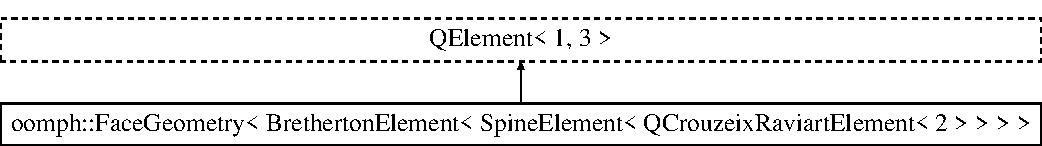
\includegraphics[height=1.958042cm]{classoomph_1_1FaceGeometry_3_01BrethertonElement_3_01SpineElement_3_01QCrouzeixRaviartElement_3_012_01_4_01_4_01_4_01_4}
\end{center}
\end{figure}
\subsection*{Public Member Functions}
\begin{DoxyCompactItemize}
\item 
\hyperlink{classoomph_1_1FaceGeometry_3_01BrethertonElement_3_01SpineElement_3_01QCrouzeixRaviartElement_3_012_01_4_01_4_01_4_01_4_a0dc4cbff5cdc502a6f653a6682cf7da5}{Face\+Geometry} ()
\end{DoxyCompactItemize}


\subsection{Detailed Description}
\subsubsection*{template$<$$>$\newline
class oomph\+::\+Face\+Geometry$<$ Bretherton\+Element$<$ Spine\+Element$<$ Q\+Crouzeix\+Raviart\+Element$<$ 2 $>$ $>$ $>$ $>$}

Face geometry of the Bretherton 2D Crouzeix\+\_\+\+Raviart spine elements. 

Definition at line 412 of file bretherton.\+cc.



\subsection{Constructor \& Destructor Documentation}
\mbox{\Hypertarget{classoomph_1_1FaceGeometry_3_01BrethertonElement_3_01SpineElement_3_01QCrouzeixRaviartElement_3_012_01_4_01_4_01_4_01_4_a0dc4cbff5cdc502a6f653a6682cf7da5}\label{classoomph_1_1FaceGeometry_3_01BrethertonElement_3_01SpineElement_3_01QCrouzeixRaviartElement_3_012_01_4_01_4_01_4_01_4_a0dc4cbff5cdc502a6f653a6682cf7da5}} 
\index{oomph\+::\+Face\+Geometry$<$ Bretherton\+Element$<$ Spine\+Element$<$ Q\+Crouzeix\+Raviart\+Element$<$ 2 $>$ $>$ $>$ $>$@{oomph\+::\+Face\+Geometry$<$ Bretherton\+Element$<$ Spine\+Element$<$ Q\+Crouzeix\+Raviart\+Element$<$ 2 $>$ $>$ $>$ $>$}!Face\+Geometry@{Face\+Geometry}}
\index{Face\+Geometry@{Face\+Geometry}!oomph\+::\+Face\+Geometry$<$ Bretherton\+Element$<$ Spine\+Element$<$ Q\+Crouzeix\+Raviart\+Element$<$ 2 $>$ $>$ $>$ $>$@{oomph\+::\+Face\+Geometry$<$ Bretherton\+Element$<$ Spine\+Element$<$ Q\+Crouzeix\+Raviart\+Element$<$ 2 $>$ $>$ $>$ $>$}}
\subsubsection{\texorpdfstring{Face\+Geometry()}{FaceGeometry()}}
{\footnotesize\ttfamily oomph\+::\+Face\+Geometry$<$ \hyperlink{classBrethertonElement}{Bretherton\+Element}$<$ Spine\+Element$<$ Q\+Crouzeix\+Raviart\+Element$<$ 2 $>$ $>$ $>$ $>$\+::Face\+Geometry (\begin{DoxyParamCaption}{ }\end{DoxyParamCaption})\hspace{0.3cm}{\ttfamily [inline]}}



Definition at line 415 of file bretherton.\+cc.



The documentation for this class was generated from the following file\+:\begin{DoxyCompactItemize}
\item 
\hyperlink{bretherton_8cc}{bretherton.\+cc}\end{DoxyCompactItemize}

\hypertarget{classoomph_1_1FaceGeometry_3_01BrethertonElement_3_01SpineElement_3_01QTaylorHoodElement_3_012_01_4_01_4_01_4_01_4}{}\section{oomph\+:\+:Face\+Geometry$<$ Bretherton\+Element$<$ Spine\+Element$<$ Q\+Taylor\+Hood\+Element$<$ 2 $>$ $>$ $>$ $>$ Class Template Reference}
\label{classoomph_1_1FaceGeometry_3_01BrethertonElement_3_01SpineElement_3_01QTaylorHoodElement_3_012_01_4_01_4_01_4_01_4}\index{oomph\+::\+Face\+Geometry$<$ Bretherton\+Element$<$ Spine\+Element$<$ Q\+Taylor\+Hood\+Element$<$ 2 $>$ $>$ $>$ $>$@{oomph\+::\+Face\+Geometry$<$ Bretherton\+Element$<$ Spine\+Element$<$ Q\+Taylor\+Hood\+Element$<$ 2 $>$ $>$ $>$ $>$}}


Face geometry of the Bretherton 2D Taylor Hood spine elements.  


Inheritance diagram for oomph\+:\+:Face\+Geometry$<$ Bretherton\+Element$<$ Spine\+Element$<$ Q\+Taylor\+Hood\+Element$<$ 2 $>$ $>$ $>$ $>$\+:\begin{figure}[H]
\begin{center}
\leavevmode
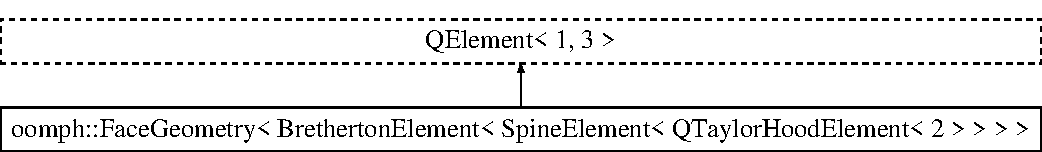
\includegraphics[height=2.000000cm]{classoomph_1_1FaceGeometry_3_01BrethertonElement_3_01SpineElement_3_01QTaylorHoodElement_3_012_01_4_01_4_01_4_01_4}
\end{center}
\end{figure}
\subsection*{Public Member Functions}
\begin{DoxyCompactItemize}
\item 
\hyperlink{classoomph_1_1FaceGeometry_3_01BrethertonElement_3_01SpineElement_3_01QTaylorHoodElement_3_012_01_4_01_4_01_4_01_4_a7dd07e5dd24aaca5c44a36cfedb04c3e}{Face\+Geometry} ()
\end{DoxyCompactItemize}


\subsection{Detailed Description}
\subsubsection*{template$<$$>$\newline
class oomph\+::\+Face\+Geometry$<$ Bretherton\+Element$<$ Spine\+Element$<$ Q\+Taylor\+Hood\+Element$<$ 2 $>$ $>$ $>$ $>$}

Face geometry of the Bretherton 2D Taylor Hood spine elements. 

Definition at line 424 of file bretherton.\+cc.



\subsection{Constructor \& Destructor Documentation}
\mbox{\Hypertarget{classoomph_1_1FaceGeometry_3_01BrethertonElement_3_01SpineElement_3_01QTaylorHoodElement_3_012_01_4_01_4_01_4_01_4_a7dd07e5dd24aaca5c44a36cfedb04c3e}\label{classoomph_1_1FaceGeometry_3_01BrethertonElement_3_01SpineElement_3_01QTaylorHoodElement_3_012_01_4_01_4_01_4_01_4_a7dd07e5dd24aaca5c44a36cfedb04c3e}} 
\index{oomph\+::\+Face\+Geometry$<$ Bretherton\+Element$<$ Spine\+Element$<$ Q\+Taylor\+Hood\+Element$<$ 2 $>$ $>$ $>$ $>$@{oomph\+::\+Face\+Geometry$<$ Bretherton\+Element$<$ Spine\+Element$<$ Q\+Taylor\+Hood\+Element$<$ 2 $>$ $>$ $>$ $>$}!Face\+Geometry@{Face\+Geometry}}
\index{Face\+Geometry@{Face\+Geometry}!oomph\+::\+Face\+Geometry$<$ Bretherton\+Element$<$ Spine\+Element$<$ Q\+Taylor\+Hood\+Element$<$ 2 $>$ $>$ $>$ $>$@{oomph\+::\+Face\+Geometry$<$ Bretherton\+Element$<$ Spine\+Element$<$ Q\+Taylor\+Hood\+Element$<$ 2 $>$ $>$ $>$ $>$}}
\subsubsection{\texorpdfstring{Face\+Geometry()}{FaceGeometry()}}
{\footnotesize\ttfamily oomph\+::\+Face\+Geometry$<$ \hyperlink{classBrethertonElement}{Bretherton\+Element}$<$ Spine\+Element$<$ Q\+Taylor\+Hood\+Element$<$ 2 $>$ $>$ $>$ $>$\+::Face\+Geometry (\begin{DoxyParamCaption}{ }\end{DoxyParamCaption})\hspace{0.3cm}{\ttfamily [inline]}}



Definition at line 427 of file bretherton.\+cc.



The documentation for this class was generated from the following file\+:\begin{DoxyCompactItemize}
\item 
\hyperlink{bretherton_8cc}{bretherton.\+cc}\end{DoxyCompactItemize}

\hypertarget{classoomph_1_1FaceGeometry_3_01FaceGeometry_3_01BrethertonElement_3_01SpineElement_3_01QCrouzeix098df2efac952001ec21ccc10b121ae7}{}\section{oomph\+:\+:Face\+Geometry$<$ Face\+Geometry$<$ Bretherton\+Element$<$ Spine\+Element$<$ Q\+Crouzeix\+Raviart\+Element$<$ 2 $>$ $>$ $>$ $>$ $>$ Class Template Reference}
\label{classoomph_1_1FaceGeometry_3_01FaceGeometry_3_01BrethertonElement_3_01SpineElement_3_01QCrouzeix098df2efac952001ec21ccc10b121ae7}\index{oomph\+::\+Face\+Geometry$<$ Face\+Geometry$<$ Bretherton\+Element$<$ Spine\+Element$<$ Q\+Crouzeix\+Raviart\+Element$<$ 2 $>$ $>$ $>$ $>$ $>$@{oomph\+::\+Face\+Geometry$<$ Face\+Geometry$<$ Bretherton\+Element$<$ Spine\+Element$<$ Q\+Crouzeix\+Raviart\+Element$<$ 2 $>$ $>$ $>$ $>$ $>$}}
Inheritance diagram for oomph\+:\+:Face\+Geometry$<$ Face\+Geometry$<$ Bretherton\+Element$<$ Spine\+Element$<$ Q\+Crouzeix\+Raviart\+Element$<$ 2 $>$ $>$ $>$ $>$ $>$\+:\begin{figure}[H]
\begin{center}
\leavevmode
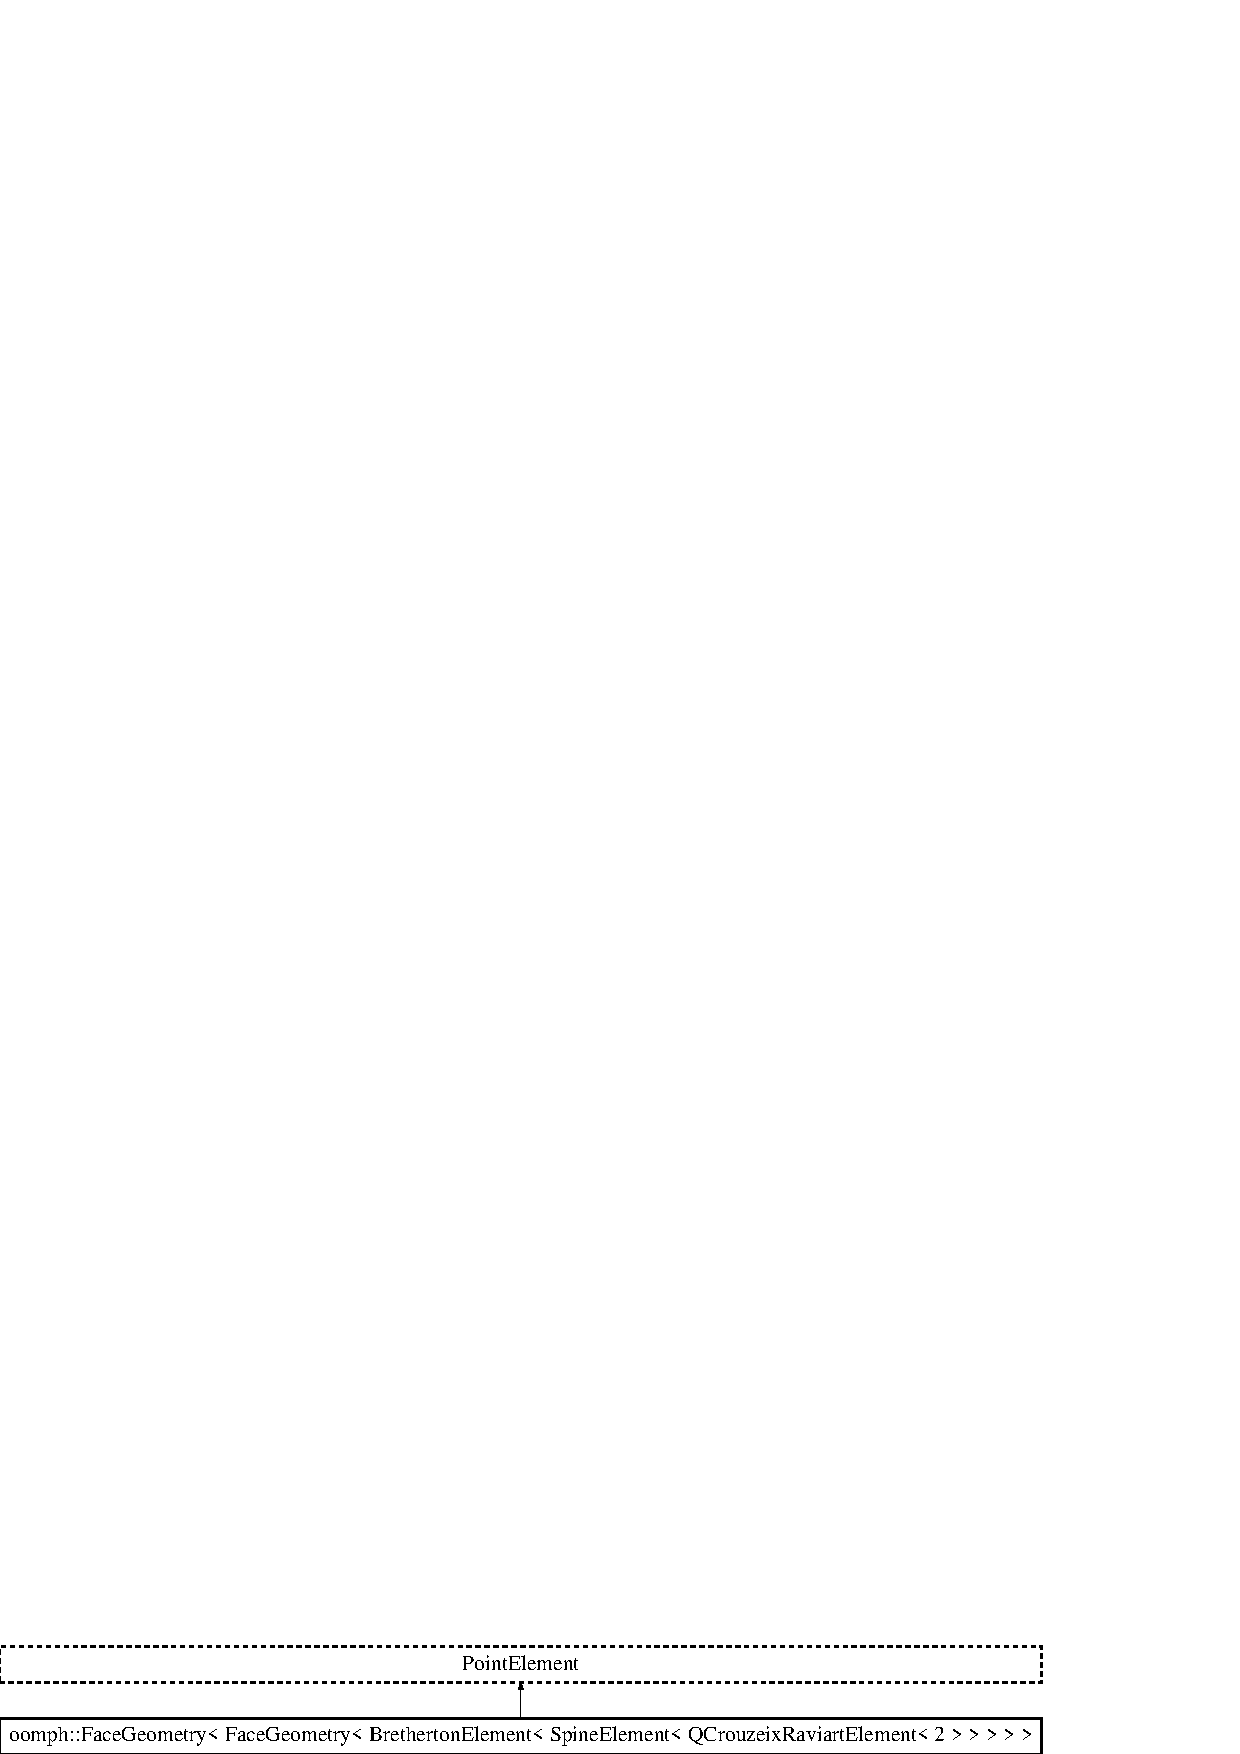
\includegraphics[height=1.649485cm]{classoomph_1_1FaceGeometry_3_01FaceGeometry_3_01BrethertonElement_3_01SpineElement_3_01QCrouzeix098df2efac952001ec21ccc10b121ae7}
\end{center}
\end{figure}
\subsection*{Public Member Functions}
\begin{DoxyCompactItemize}
\item 
\hyperlink{classoomph_1_1FaceGeometry_3_01FaceGeometry_3_01BrethertonElement_3_01SpineElement_3_01QCrouzeix098df2efac952001ec21ccc10b121ae7_a52eb404b07af95adc77be5b560f7186b}{Face\+Geometry} ()
\end{DoxyCompactItemize}


\subsection{Detailed Description}
\subsubsection*{template$<$$>$\newline
class oomph\+::\+Face\+Geometry$<$ Face\+Geometry$<$ Bretherton\+Element$<$ Spine\+Element$<$ Q\+Crouzeix\+Raviart\+Element$<$ 2 $>$ $>$ $>$ $>$ $>$}

Face geometry of the Face geometry of the the Bretherton 2D Crouzeix\+\_\+\+Raviart spine elements 

Definition at line 436 of file bretherton.\+cc.



\subsection{Constructor \& Destructor Documentation}
\mbox{\Hypertarget{classoomph_1_1FaceGeometry_3_01FaceGeometry_3_01BrethertonElement_3_01SpineElement_3_01QCrouzeix098df2efac952001ec21ccc10b121ae7_a52eb404b07af95adc77be5b560f7186b}\label{classoomph_1_1FaceGeometry_3_01FaceGeometry_3_01BrethertonElement_3_01SpineElement_3_01QCrouzeix098df2efac952001ec21ccc10b121ae7_a52eb404b07af95adc77be5b560f7186b}} 
\index{oomph\+::\+Face\+Geometry$<$ Face\+Geometry$<$ Bretherton\+Element$<$ Spine\+Element$<$ Q\+Crouzeix\+Raviart\+Element$<$ 2 $>$ $>$ $>$ $>$ $>$@{oomph\+::\+Face\+Geometry$<$ Face\+Geometry$<$ Bretherton\+Element$<$ Spine\+Element$<$ Q\+Crouzeix\+Raviart\+Element$<$ 2 $>$ $>$ $>$ $>$ $>$}!Face\+Geometry@{Face\+Geometry}}
\index{Face\+Geometry@{Face\+Geometry}!oomph\+::\+Face\+Geometry$<$ Face\+Geometry$<$ Bretherton\+Element$<$ Spine\+Element$<$ Q\+Crouzeix\+Raviart\+Element$<$ 2 $>$ $>$ $>$ $>$ $>$@{oomph\+::\+Face\+Geometry$<$ Face\+Geometry$<$ Bretherton\+Element$<$ Spine\+Element$<$ Q\+Crouzeix\+Raviart\+Element$<$ 2 $>$ $>$ $>$ $>$ $>$}}
\subsubsection{\texorpdfstring{Face\+Geometry()}{FaceGeometry()}}
{\footnotesize\ttfamily oomph\+::\+Face\+Geometry$<$ Face\+Geometry$<$ \hyperlink{classBrethertonElement}{Bretherton\+Element}$<$ Spine\+Element$<$ Q\+Crouzeix\+Raviart\+Element$<$ 2 $>$ $>$ $>$ $>$ $>$\+::Face\+Geometry (\begin{DoxyParamCaption}{ }\end{DoxyParamCaption})\hspace{0.3cm}{\ttfamily [inline]}}



Definition at line 440 of file bretherton.\+cc.



The documentation for this class was generated from the following file\+:\begin{DoxyCompactItemize}
\item 
\hyperlink{bretherton_8cc}{bretherton.\+cc}\end{DoxyCompactItemize}

\hypertarget{classoomph_1_1FaceGeometry_3_01FaceGeometry_3_01BrethertonElement_3_01SpineElement_3_01QTaylorHoa5ee68c3d3e62f3e07a972f1f9faface}{}\section{oomph\+:\+:Face\+Geometry$<$ Face\+Geometry$<$ Bretherton\+Element$<$ Spine\+Element$<$ Q\+Taylor\+Hood\+Element$<$ 2 $>$ $>$ $>$ $>$ $>$ Class Template Reference}
\label{classoomph_1_1FaceGeometry_3_01FaceGeometry_3_01BrethertonElement_3_01SpineElement_3_01QTaylorHoa5ee68c3d3e62f3e07a972f1f9faface}\index{oomph\+::\+Face\+Geometry$<$ Face\+Geometry$<$ Bretherton\+Element$<$ Spine\+Element$<$ Q\+Taylor\+Hood\+Element$<$ 2 $>$ $>$ $>$ $>$ $>$@{oomph\+::\+Face\+Geometry$<$ Face\+Geometry$<$ Bretherton\+Element$<$ Spine\+Element$<$ Q\+Taylor\+Hood\+Element$<$ 2 $>$ $>$ $>$ $>$ $>$}}
Inheritance diagram for oomph\+:\+:Face\+Geometry$<$ Face\+Geometry$<$ Bretherton\+Element$<$ Spine\+Element$<$ Q\+Taylor\+Hood\+Element$<$ 2 $>$ $>$ $>$ $>$ $>$\+:\begin{figure}[H]
\begin{center}
\leavevmode
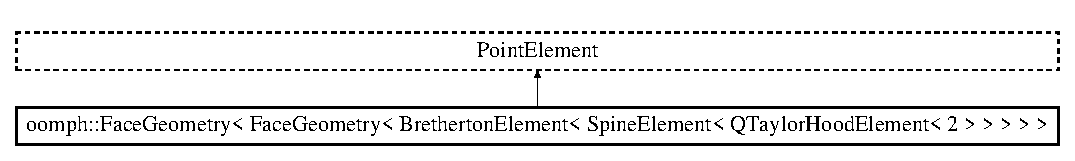
\includegraphics[height=1.709924cm]{classoomph_1_1FaceGeometry_3_01FaceGeometry_3_01BrethertonElement_3_01SpineElement_3_01QTaylorHoa5ee68c3d3e62f3e07a972f1f9faface}
\end{center}
\end{figure}
\subsection*{Public Member Functions}
\begin{DoxyCompactItemize}
\item 
\hyperlink{classoomph_1_1FaceGeometry_3_01FaceGeometry_3_01BrethertonElement_3_01SpineElement_3_01QTaylorHoa5ee68c3d3e62f3e07a972f1f9faface_a35e4c88e39164f318d20e3c7e4ddadc1}{Face\+Geometry} ()
\end{DoxyCompactItemize}


\subsection{Detailed Description}
\subsubsection*{template$<$$>$\newline
class oomph\+::\+Face\+Geometry$<$ Face\+Geometry$<$ Bretherton\+Element$<$ Spine\+Element$<$ Q\+Taylor\+Hood\+Element$<$ 2 $>$ $>$ $>$ $>$ $>$}

Face geometry of face geometry of the Bretherton 2D Taylor Hood spine elements 

Definition at line 450 of file bretherton.\+cc.



\subsection{Constructor \& Destructor Documentation}
\mbox{\Hypertarget{classoomph_1_1FaceGeometry_3_01FaceGeometry_3_01BrethertonElement_3_01SpineElement_3_01QTaylorHoa5ee68c3d3e62f3e07a972f1f9faface_a35e4c88e39164f318d20e3c7e4ddadc1}\label{classoomph_1_1FaceGeometry_3_01FaceGeometry_3_01BrethertonElement_3_01SpineElement_3_01QTaylorHoa5ee68c3d3e62f3e07a972f1f9faface_a35e4c88e39164f318d20e3c7e4ddadc1}} 
\index{oomph\+::\+Face\+Geometry$<$ Face\+Geometry$<$ Bretherton\+Element$<$ Spine\+Element$<$ Q\+Taylor\+Hood\+Element$<$ 2 $>$ $>$ $>$ $>$ $>$@{oomph\+::\+Face\+Geometry$<$ Face\+Geometry$<$ Bretherton\+Element$<$ Spine\+Element$<$ Q\+Taylor\+Hood\+Element$<$ 2 $>$ $>$ $>$ $>$ $>$}!Face\+Geometry@{Face\+Geometry}}
\index{Face\+Geometry@{Face\+Geometry}!oomph\+::\+Face\+Geometry$<$ Face\+Geometry$<$ Bretherton\+Element$<$ Spine\+Element$<$ Q\+Taylor\+Hood\+Element$<$ 2 $>$ $>$ $>$ $>$ $>$@{oomph\+::\+Face\+Geometry$<$ Face\+Geometry$<$ Bretherton\+Element$<$ Spine\+Element$<$ Q\+Taylor\+Hood\+Element$<$ 2 $>$ $>$ $>$ $>$ $>$}}
\subsubsection{\texorpdfstring{Face\+Geometry()}{FaceGeometry()}}
{\footnotesize\ttfamily oomph\+::\+Face\+Geometry$<$ Face\+Geometry$<$ \hyperlink{classBrethertonElement}{Bretherton\+Element}$<$ Spine\+Element$<$ Q\+Taylor\+Hood\+Element$<$ 2 $>$ $>$ $>$ $>$ $>$\+::Face\+Geometry (\begin{DoxyParamCaption}{ }\end{DoxyParamCaption})\hspace{0.3cm}{\ttfamily [inline]}}



Definition at line 453 of file bretherton.\+cc.



The documentation for this class was generated from the following file\+:\begin{DoxyCompactItemize}
\item 
\hyperlink{bretherton_8cc}{bretherton.\+cc}\end{DoxyCompactItemize}

\chapter{File Documentation}
\hypertarget{bretherton_8cc}{}\section{bretherton.\+cc File Reference}
\label{bretherton_8cc}\index{bretherton.\+cc@{bretherton.\+cc}}
\subsection*{Classes}
\begin{DoxyCompactItemize}
\item 
class \hyperlink{classBrethertonElement}{Bretherton\+Element$<$ E\+L\+E\+M\+E\+N\+T $>$}
\item 
class \hyperlink{classoomph_1_1FaceGeometry_3_01BrethertonElement_3_01SpineElement_3_01QCrouzeixRaviartElement_3_012_01_4_01_4_01_4_01_4}{oomph\+::\+Face\+Geometry$<$ Bretherton\+Element$<$ Spine\+Element$<$ Q\+Crouzeix\+Raviart\+Element$<$ 2 $>$ $>$ $>$ $>$}
\begin{DoxyCompactList}\small\item\em Face geometry of the Bretherton 2D Crouzeix\+\_\+\+Raviart spine elements. \end{DoxyCompactList}\item 
class \hyperlink{classoomph_1_1FaceGeometry_3_01BrethertonElement_3_01SpineElement_3_01QTaylorHoodElement_3_012_01_4_01_4_01_4_01_4}{oomph\+::\+Face\+Geometry$<$ Bretherton\+Element$<$ Spine\+Element$<$ Q\+Taylor\+Hood\+Element$<$ 2 $>$ $>$ $>$ $>$}
\begin{DoxyCompactList}\small\item\em Face geometry of the Bretherton 2D Taylor Hood spine elements. \end{DoxyCompactList}\item 
class \hyperlink{classoomph_1_1FaceGeometry_3_01FaceGeometry_3_01BrethertonElement_3_01SpineElement_3_01QCrouzeix098df2efac952001ec21ccc10b121ae7}{oomph\+::\+Face\+Geometry$<$ Face\+Geometry$<$ Bretherton\+Element$<$ Spine\+Element$<$ Q\+Crouzeix\+Raviart\+Element$<$ 2 $>$ $>$ $>$ $>$ $>$}
\item 
class \hyperlink{classoomph_1_1FaceGeometry_3_01FaceGeometry_3_01BrethertonElement_3_01SpineElement_3_01QTaylorHoa5ee68c3d3e62f3e07a972f1f9faface}{oomph\+::\+Face\+Geometry$<$ Face\+Geometry$<$ Bretherton\+Element$<$ Spine\+Element$<$ Q\+Taylor\+Hood\+Element$<$ 2 $>$ $>$ $>$ $>$ $>$}
\item 
class \hyperlink{classBrethertonProblem}{Bretherton\+Problem$<$ E\+L\+E\+M\+E\+N\+T $>$}
\begin{DoxyCompactList}\small\item\em Bretherton problem. \end{DoxyCompactList}\end{DoxyCompactItemize}
\subsection*{Namespaces}
\begin{DoxyCompactItemize}
\item 
 \hyperlink{namespaceGlobal__Physical__Variables}{Global\+\_\+\+Physical\+\_\+\+Variables}
\begin{DoxyCompactList}\small\item\em Namepspace for global parameters. \end{DoxyCompactList}\item 
 \hyperlink{namespaceoomph}{oomph}
\end{DoxyCompactItemize}
\subsection*{Functions}
\begin{DoxyCompactItemize}
\item 
Vector$<$ double $>$ \hyperlink{namespaceGlobal__Physical__Variables_a18fe245262ec8beec764c805bb93e73c}{Global\+\_\+\+Physical\+\_\+\+Variables\+::G} (2)
\begin{DoxyCompactList}\small\item\em Direction of gravity. \end{DoxyCompactList}\item 
void \hyperlink{namespaceGlobal__Physical__Variables_a08e9835d71b7f7194ec5475f139211be}{Global\+\_\+\+Physical\+\_\+\+Variables\+::inflow} (const Vector$<$ double $>$ \&x, Vector$<$ double $>$ \&veloc)
\item 
int \hyperlink{bretherton_8cc_a0ddf1224851353fc92bfbff6f499fa97}{main} (int argc, char $\ast$argv\mbox{[}$\,$\mbox{]})
\end{DoxyCompactItemize}
\subsection*{Variables}
\begin{DoxyCompactItemize}
\item 
double \hyperlink{namespaceGlobal__Physical__Variables_ab814e627d2eb5bc50318879d19ab16b9}{Global\+\_\+\+Physical\+\_\+\+Variables\+::\+Re}
\begin{DoxyCompactList}\small\item\em Reynolds number. \end{DoxyCompactList}\item 
double \hyperlink{namespaceGlobal__Physical__Variables_a085ee4bf968ffdd01a41b8c41864f907}{Global\+\_\+\+Physical\+\_\+\+Variables\+::\+Re\+St}
\begin{DoxyCompactList}\small\item\em Womersley = Reynolds times Strouhal. \end{DoxyCompactList}\item 
double \hyperlink{namespaceGlobal__Physical__Variables_aa6286f02b476912dd7550eced538331a}{Global\+\_\+\+Physical\+\_\+\+Variables\+::\+Re\+Inv\+Fr}
\begin{DoxyCompactList}\small\item\em Product of Reynolds and Froude number. \end{DoxyCompactList}\item 
double \hyperlink{namespaceGlobal__Physical__Variables_a8b32b93d2e546f9375ec418474107838}{Global\+\_\+\+Physical\+\_\+\+Variables\+::\+Ca}
\begin{DoxyCompactList}\small\item\em Capillary number. \end{DoxyCompactList}\item 
double $\ast$ \hyperlink{namespaceGlobal__Physical__Variables_a137bdac2ad4b72a03ec9916e8ee7395b}{Global\+\_\+\+Physical\+\_\+\+Variables\+::\+H\+\_\+lo\+\_\+pt}
\begin{DoxyCompactList}\small\item\em Pointer to film thickness at outflow on the lower wall. \end{DoxyCompactList}\item 
double $\ast$ \hyperlink{namespaceGlobal__Physical__Variables_a83a3a82f89784013805bd23d63faa7e3}{Global\+\_\+\+Physical\+\_\+\+Variables\+::\+H\+\_\+up\+\_\+pt}
\begin{DoxyCompactList}\small\item\em Pointer to film thickness at outflow on the upper wall. \end{DoxyCompactList}\item 
double $\ast$ \hyperlink{namespaceGlobal__Physical__Variables_a84caa2a64e50ba5b390a3cd100f0f835}{Global\+\_\+\+Physical\+\_\+\+Variables\+::\+Y\+\_\+lo\+\_\+pt}
\begin{DoxyCompactList}\small\item\em Pointer to y-\/position at inflow on the lower wall. \end{DoxyCompactList}\item 
double $\ast$ \hyperlink{namespaceGlobal__Physical__Variables_a75878a0c79c88065fd9031f273b62698}{Global\+\_\+\+Physical\+\_\+\+Variables\+::\+Y\+\_\+up\+\_\+pt}
\begin{DoxyCompactList}\small\item\em Pointer to y-\/position at inflow on the upper wall. \end{DoxyCompactList}\end{DoxyCompactItemize}


\subsection{Function Documentation}
\mbox{\Hypertarget{bretherton_8cc_a0ddf1224851353fc92bfbff6f499fa97}\label{bretherton_8cc_a0ddf1224851353fc92bfbff6f499fa97}} 
\index{bretherton.\+cc@{bretherton.\+cc}!main@{main}}
\index{main@{main}!bretherton.\+cc@{bretherton.\+cc}}
\subsubsection{\texorpdfstring{main()}{main()}}
{\footnotesize\ttfamily int main (\begin{DoxyParamCaption}\item[{int}]{argc,  }\item[{char $\ast$}]{argv\mbox{[}$\,$\mbox{]} }\end{DoxyParamCaption})}

Driver code for unsteady two-\/layer fluid problem. If there are any command line arguments, we regard this as a validation run and perform only a single step. 

Definition at line 920 of file bretherton.\+cc.



References Global\+\_\+\+Physical\+\_\+\+Variables\+::\+Ca, Global\+\_\+\+Physical\+\_\+\+Variables\+::\+G(), Bretherton\+Problem$<$ E\+L\+E\+M\+E\+N\+T $>$\+::parameter\+\_\+study(), Global\+\_\+\+Physical\+\_\+\+Variables\+::\+Re, Global\+\_\+\+Physical\+\_\+\+Variables\+::\+Re\+Inv\+Fr, and Global\+\_\+\+Physical\+\_\+\+Variables\+::\+Re\+St.


\hypertarget{bretherton_8txt__doxygenified_8h}{}\section{bretherton.\+txt\+\_\+doxygenified.\+h File Reference}
\label{bretherton_8txt__doxygenified_8h}\index{bretherton.\+txt\+\_\+doxygenified.\+h@{bretherton.\+txt\+\_\+doxygenified.\+h}}

%--- End generated contents ---

% Index
\backmatter
\newpage
\phantomsection
\clearemptydoublepage
\addcontentsline{toc}{chapter}{Index}
\printindex

\end{document}
